\chapter{Integrais Múltiplas}

\section{Integrais Duplas sobre Retângulos}

Se $f(x)$ é uma função de uma única variável real e é definida para $a \le x \le b$, subdividimos o intervalo $[a,b]$ em $n$ subintervalos $[x_{i-1},x_i]$ de comprimento igual a $\Delta x = (b-a)/n$ e escolhemos pontos arbitrários $x_i^{*}$ em cada um desses intervalos. Em seguida, formamos a soma de Riemann e tomamos o limite dessa soma quando $n \rightarrow \infty$ para oter a integral definida de $a$ até $b$ da função $f$

\begin{equation}
\lim_{n \rightarrow \infty} \sum_{i=1}^n f(x_i^*) \cdot \Delta x = \int_a^b f(x) dx
\end{equation}

\begin{figure}[!h]
 \centering
 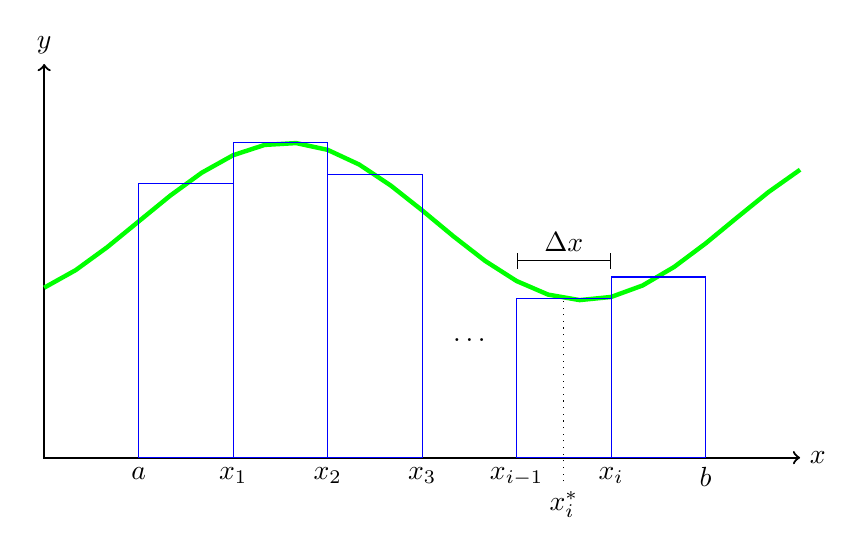
\begin{tikzpicture}[xscale=1.2]
 %\draw [help lines] (0,0) grid (8,5);
 \draw [<->, thick] (0,5) -- (0,0) -- (8,0);
 \node [above] at (0,5) {$y$}; \node [right] at (8,0) {$x$}; 
 \draw[green, ultra thick, domain=0:8] plot (\x, {3+sin(deg(\x - 1))});
 \draw [blue] (1,0) rectangle (2,3.4794);
 \node [below] at (1,0) {$a$};
 \draw [blue] (2,0) rectangle (3,3.9975);
 \node [below] at (2,0) {$x_1$};
 \draw [blue] (3,0) rectangle (4,3.5985);
 \node [below] at (3,0) {$x_2$};
 \node [below] at (4,0) {$x_3$};
 \node at (4.5,1.5) {$\ldots$};
 \draw [blue] (5,0) rectangle (6,2.0225);
 \node [below] at (5,0) {$x_{i-1}$};
 \node [below] at (6,0) {$x_{i}$};
 \draw [blue] (6,0) rectangle (7,2.2945);
 \node [below] at (7,0) {$b$};
 \draw [|-|] (5,2.5) -- (6,2.5); \node [above] at (5.5,2.5) {$\Delta x$};
 \node [below=.3cm] at (5.5,0) {$x_i^*$};
 \draw [dotted] (5.5,-.3) -- (5.5,2.0225);
\end{tikzpicture}
 \caption{Somas de Riemman para funções de uma variável}
\end{figure}

De modo semelhante, considere uma função $f$ de duas variáveis definida em um retângulo fechado.

$$R = [a,b] \times [c,d] = \{ (x,y) \in \mathbb{R}^2 | a \le x \le b, c \le y \le d \} $$

O gráfico de $f$ é a superfície com equação $z = f(x,y)$. Seja $S$ o sólido contido acima de $R$ e abaixo da superfície $z$:

$$ S = \{ (x,y,z) \in  \mathbb{R}^3 | 0 \le z \le f(x,y), (x,y) \in R \} $$

\begin{figure}[!h]
 \centering
 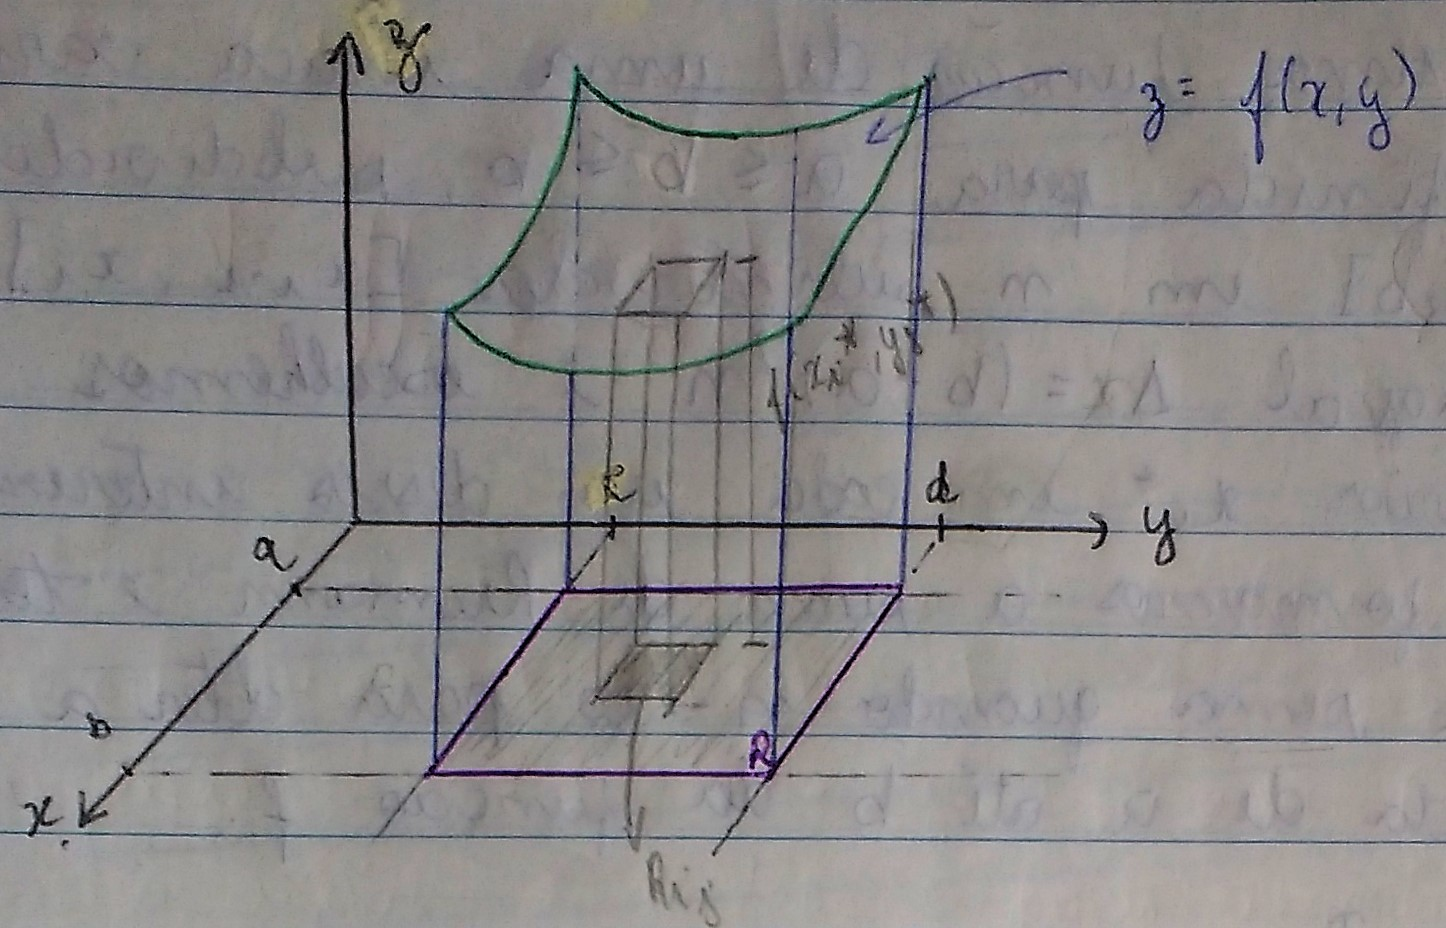
\includegraphics[width=10cm]{Pictures/graph2.jpg}
\end{figure}

Para determinar o volume de $S$, o primeiro passo é dividir o retângulo $R$ em sub-retângulos. Faremos isto dividindo o intervalo $[a,b]$ em $m$ subintervalos $[x_{i-1}, x_{i}]$ de mesmo comprimento $\delta x = (b-a)/m$ e o intervalo $[c,d]$ em $n$ subintervalos iguais $[y_{j-1}, y_{j}]$ de comprimento $\delta y = (d-c)/n$.

\begin{figure}[!h]
 \centering
 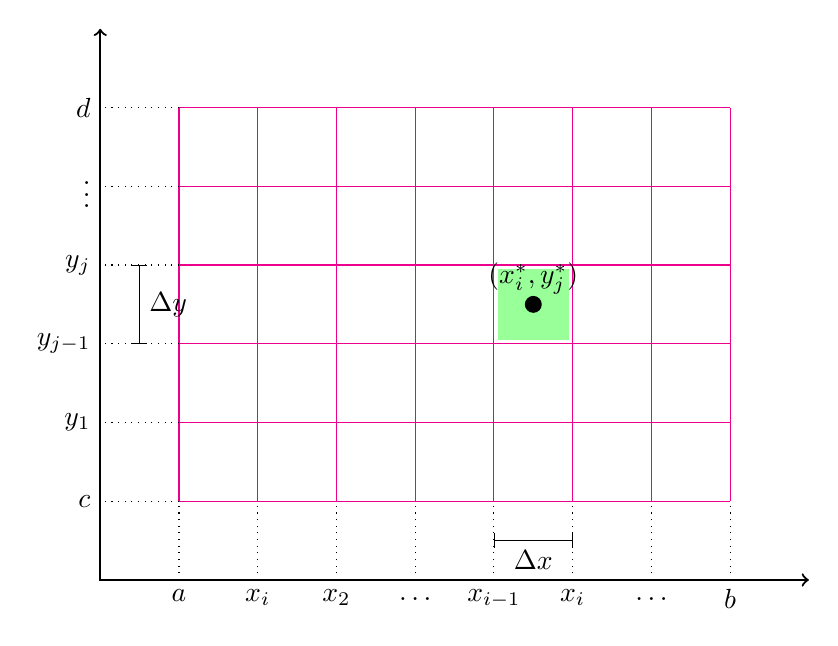
\begin{tikzpicture}
 %\draw [help lines] (0,0) grid (9,7);
 \draw [<->, thick] (0,7) -- (0,0) -- (9,0);
 %\node [above] at (0,5) {$y$}; \node [right] at (8,0) {$x$};
 \foreach \i in {1,...,8}
 {
  \draw [magenta] (\i,1) -- (\i,6);
  \draw [dotted] (\i,0) -- (\i,1);
 }
 \node [below] at (1,0) {$a$};
 \node [below] at (2,0) {$x_i$};
 \node [below] at (3,0) {$x_2$};
 \node [below=.1cm] at (4,0) {$\ldots$};
 \node [below] at (5,0) {$x_{i-1}$};
 \node [below=.1cm] at (7,0) {$\ldots$};
 \node [below] at (6,0) {$x_i$};
 \node [below] at (8,0) {$b$};
 \foreach \i in {1,...,6}
 {
  \draw [magenta] (1,\i) -- (8,\i);
  \draw [dotted] (1,\i) -- (0,\i);
 }
 \node [left] at (0,1) {$c$};
 \node [left] at (0,2) {$y_1$};
 \node [left] at (0,3) {$y_{j-1}$};
 \node [left] at (0,4) {$y_j$};
 \node [left] at (0,5) {$\vdots$};
 \node [left] at (0,6) {$d$};
 % labels y
 \path [fill=green!40] (5.05,3.05) rectangle (5.95,3.95);
 \draw [fill] (5.5,3.5) circle [radius=.1] node [above] {$(x_i^*, y_j^*)$};
 \draw [|-|] (5,0.5) -- (6,0.5); \node [below] at (5.5,0.5) {$\Delta x$};
 \draw [|-|] (0.5,3) -- (0.5,4); \node [right] at (0.5,3.5) {$\Delta y$};
\end{tikzpicture}
\end{figure}

Se escolhermos um ponto arbitrário em cada $R_{ij}$, $(x_i^*, y_j^*)$ definimos o volume da caixa de base $R_{ij}$ e altura $f(x_i^*, y_j^*)$ como:

$$ f(x_i^*, y_j^*) \cdot \Delta A $$

Se realizarmos este procedimento para os demais retângulos, vamos obter uma estimativa do volume:

$$ V \approx \sum_{i=1}^m \sum{j=1}^n f(x_i^*, y_j^*) \cdot \Delta A $$

A aproximação do volume acima melhora quando aumentamos os valores de $m$ e $n$, portanto:

$$ V = \lim_{m,n \rightarrow \infty} \sum_{i=1}^m \sum{j=1}^n f(x_i^*, y_j^*) \cdot \Delta A $$

Daí, podemos enunciar a definição de integral dupla sobre um retângulo $R_{ij}$.

\begin{definition}[Integral Dupla]
 A integral dupla de $f$ sobre o retângulo $R_{ij}$ é:
 \begin{equation}
  \iint _{R} f(x,y) dA = \lim_{m,n \rightarrow \infty} \sum_{i=1}^m \sum{j=1}^n f(x_i^*, y_j^*) \cdot \Delta A
 \end{equation}
 se este limite existir.
\end{definition}

O significado preciso da definição anterior é que para todo $\epsilon > 0$, existe um número $N$ talque

$$ \| \iint _{R} f(x,y) dA -  \lim_{m,n \rightarrow \infty} \sum_{i=1}^m \sum{j=1}^n f(x_i^*, y_j^*) \cdot \Delta A \| < \epsilon $$

para todos inteiros $m$ e $n$ maiores que $N$ e para qualquer escolha de $(x_i^*, y_j^*)$ em $R_{ij}$.

